\chapter{Related work (State-of-the-art)}
In this chapter we would like to introduce some related works,which propose different approaches to the problem of detection and classification of intracranial hemorrhage in non-contrast CT scans.

\section{Identification of intracranial hemorrhage with clinical workflow integration}
In their work \cite{relatedWork1}, Arbabshirani et al. developed a machine learning algorithm, which automatically analyzed head CT scans, flagging those with the presence of a hemorrhage, and thus prioritized radiology work lists in real time. As a result, it became possible to significantly reduce the average time, in which a patient received their diagnosis.  
\subsection*{Methods} 
The machine learning algorithm implemented in this study was a three-dimensional convolutional neural network, with the architecture of five convolutional layers and two fully connected layers. The dataset used in development of the solution contained 46 583 non-contrast head CT studies, each having 20 axial two-dimensional slices. Each study had been manually labeled with a binary value, signalizing the presence of a hemorrhage. These labels were later used as ground truths during training phase. Prior to the network training, the data had been preprocessed with several techniques, such as standardizing the number of axial slices and resizing each slice, so to achieve a uniform dimensions of 256x256x24 for each study, as well as applying windowing, in order to increase the contrast in each of the slices. Thenceforth, the neural network was trained using stochastic gradient descent, until the received loss was near zero. After the training period, the algorithm was tested on previously unseen test data.
\subsection*{Clinical implementation} 
Over a three-month period, the trained model had been implemented at a clinic in Pennsylvania, USA to assist with prioritization of radiology work lists. During this implementation phase, 347 head CT studies were processed in real time. For each study, which was fed to the algorithm, a binary output was produced, representing positive or negative presence of ICH. Studies marked as positive were assigned higher priority and moved up the radiology work list. Out of these 94 studies, 60 were determined by a interpreting radiologist as true positive, which gave the model positive predictive value of 64\%. were consequently . With this approach, average diagnostic time was shortened from 8,5 hours to just 19 minutes, which is acceleration of 96\%. The algorithm showed accuracy of 84\% sensitivity of 70\%  and specificity of 87\%. The area under the curve of the model, was established to be 0.846.
\begin{figure}[!ht]
\begin{centering}
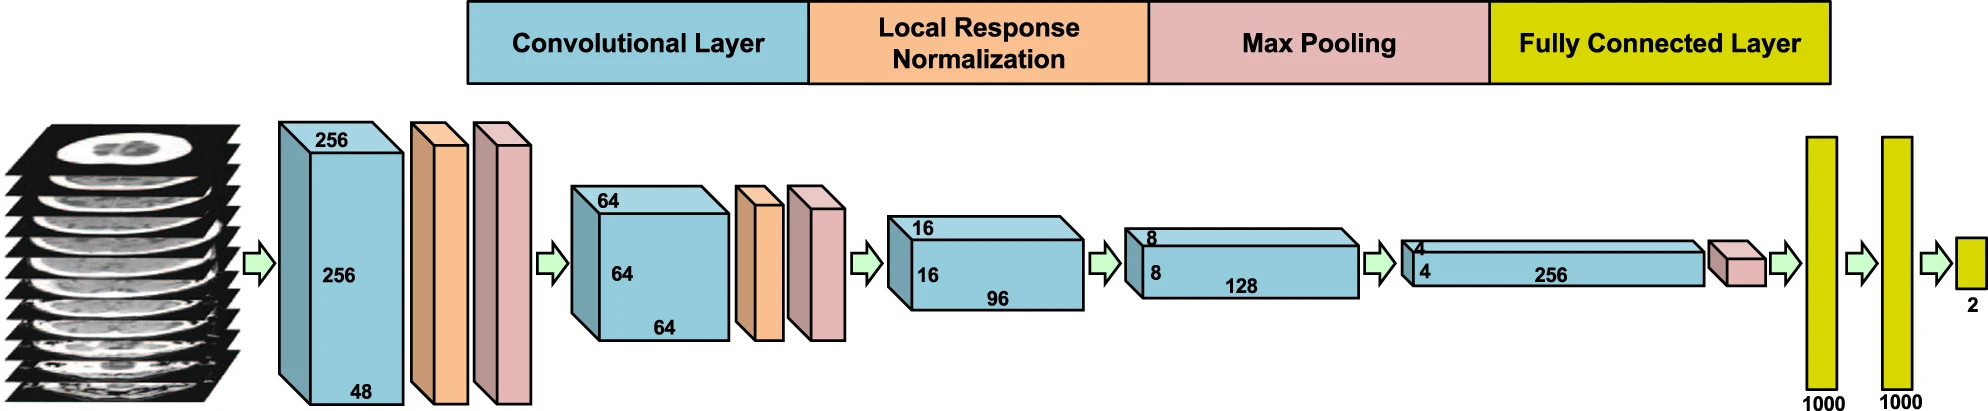
\includegraphics[width=16cm]{assets/images/RW1-net-arch.png}
\par\end{centering}
\caption{Model architecture from \footfullcite{relatedWork1} \label{fig:rw1}}
\end{figure}

\section{Diagnosis of intracranial hemorrhage and subtypes using a three-dimensional joint convolutional and recurrent neural network}

The work of Ye et al. \cite{relatedWork2} resides in combining three-dimensional joint convolutional neural network (CNN) and recurrent neural network (RNN) for the task of detecting intracranial hemorrhage, as well as its five subtypes. The authors conducted a comparison and evaluation of their solution on both slice-level and subject-level (whole 3D CT scan) approaches.

\subsection*{Dataset}
Dataset containing 2836 non-contrast head CT scans was used, out of which 1836 scans were with positive appearance of intracranial hemorrhage. The remaining 1000 scans had been labeled as healthy, without any hemorrhage. All of the scans were labeled on both, slice - and subject - levels. Typically, data preprocessing forewent the training process. This included resampling and downsampling the original dimensions of the scans. Just like in the previously mentioned study \cite{relatedWork1}, different types of windowing were applied on slice-level. Peprocessed data were then used in two stage training. 
\subsection*{Methods}
During the first stage, a two-type classification was conducted, which predicted the very presence of a bleeding. With this step, every subject not containing intracranial hemorrhage was filtered out, and only the subjects with bleeding occuring were forwarded to the second stage. In this stage, five-type classification determined the subtype of the hemorrhage present in the scan. The convolutional neural network was trained to serve as a feature extractor on a slice level. Followed by a reccurent neural network, which was implemented to "capture sequential information of features from consecutive slices, adding inter-slice dependency context to boost classification performance" \cite{relatedWork2}. To introduce some explainability and review the regions upon which their model made predictions, authors used the Grad-CAM method, which generated heatmaps based on most relevant regions of input images.
\begin{figure}[!ht]
\begin{centering}
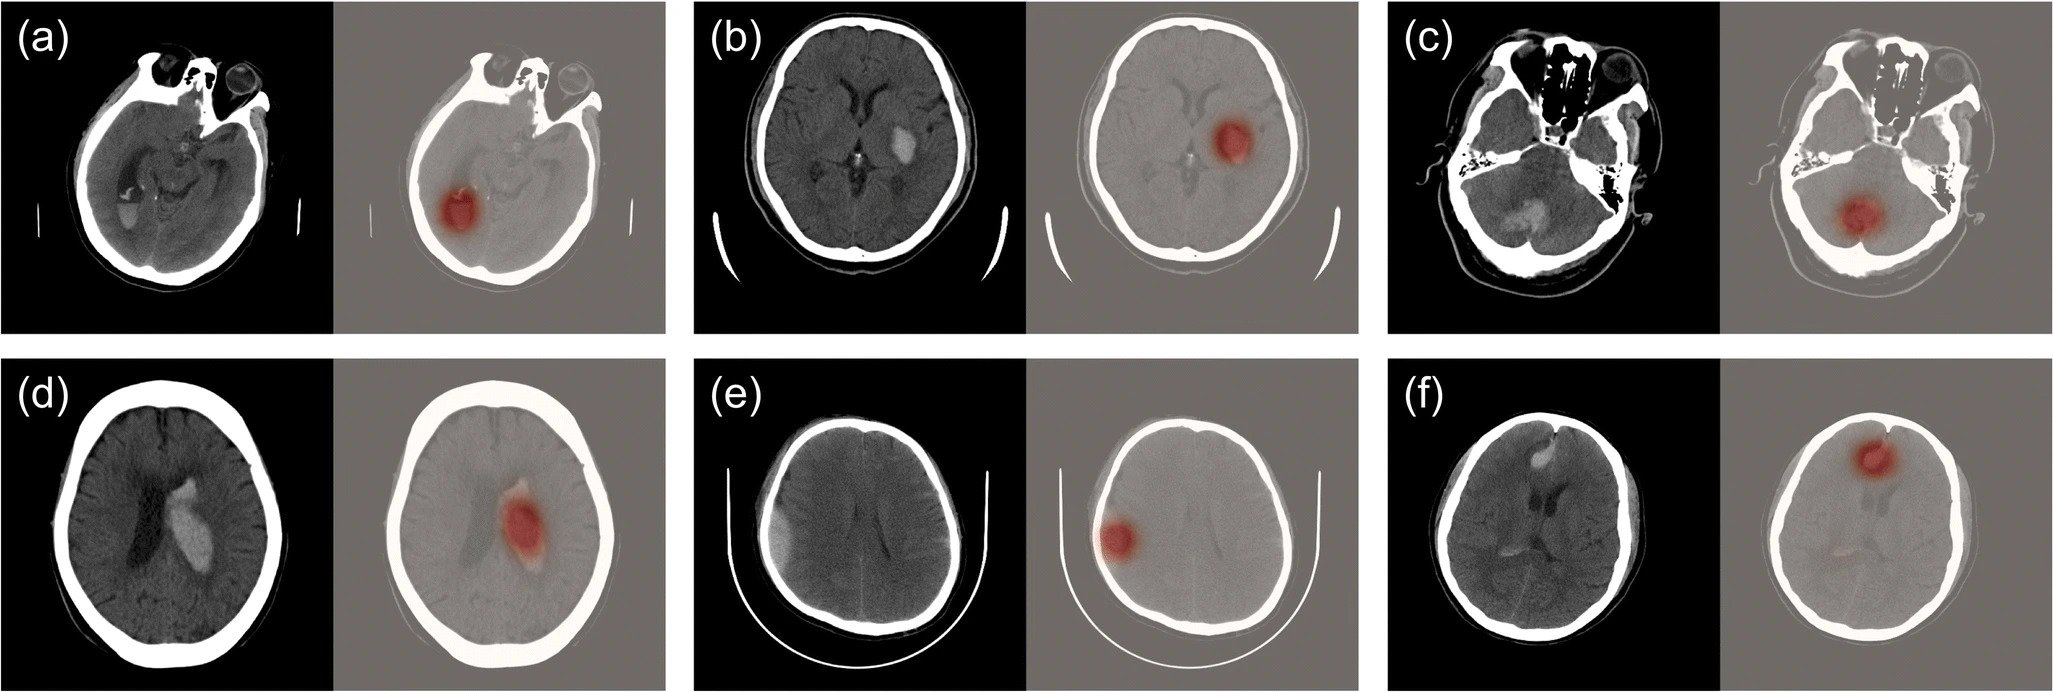
\includegraphics[width=15cm]{assets/images/RW2.jpg}
\par\end{centering}
\caption{Heatmpas generated with the Grad-CAM \footfullcite{relatedWork2} \label{fig:rw2}}
\end{figure}

\section{}